\documentclass{beamer}
\usepackage[utf8x]{inputenc}

\usepackage{color}
\usepackage{xcolor}

\definecolor{solarbg}{HTML}{FDF6E3}
\definecolor{Green}{HTML}{00BB00}

\usepackage{minted}
\newminted{java}{bgcolor=solarbg,frame=single}
\newminted{clj}{bgcolor=solarbg,frame=single}
\newminted{py}{bgcolor=solarbg,frame=single}
\usemintedstyle{solarized}

\usetheme{Antibes}
\usecolortheme[named=Green]{structure}

\titlegraphic{
\includegraphics[scale=0.75]{img/clj.pdf}}
\title[Introduksjonskurs til programmeringsspråket Clo{\em j}ure]{Kurs i Clo{\em j}ure}
\author{Jean Niklas L'orange}
\institute{\texttt{jeannikl@hypirion.com}}
\date{16. oktober, 2012}

\begin{document}

\begin{frame}
  \titlepage
\end{frame}

\section{Hva er Clojure?}

\begin{frame}
  \frametitle{Hva er Clojure?}
  \begin{itemize}
  \item<1-> Dynamisk
    \begin{itemize}
      \item<2-> en ny lisp, ikke Scheme eller Common Lisp
    \end{itemize}
  \item<3-> Funksjonelt
    \begin{itemize}
      \item<4-> med fokus på immutabilitet
    \end{itemize}
  \item<5-> Designet for ``flertråding''
  \item<6-> Kjører på Java VM
    \begin{itemize}
      \item<7-> kompilerer ned til Java bytekode
    \end{itemize}
  \item<8-> Ikke objektorientert 
  \end{itemize}
\end{frame}

\section{Motivasjon}

\begin{frame}
  \frametitle{Motivasjon}
  \framesubtitle{Hvorfor burde man lære seg Clojure?}
  \begin{itemize}
    \item<1-> Lett(ere) å lese og forstå kode
    \item<2-> Designet for programmering med flere tråder
    \item<3-> Har et REPL - lettere å teste/lære språket
    \item<4-> Transaksjonsbasert minne
    \item<5-> Lettere å innføre enn andre språk der du jobber
    \item<6-> Mer morsomt enn andre språk! (Forhåpentligvis)
  \end{itemize}
\end{frame}

\begin{frame}[fragile]
  \frametitle{Lett(ere) å lese kode}

  Hello world i Java:
  \vspace{3mm}
  \begin{javacode}
public class HelloWorld {
  public static void main(String[] args){
    System.out.println("Hello world!");
  }
}
  \end{javacode}

  versus hello world i Clojure*
  \vspace{3mm}
  \begin{cljcode}
(defn -main [& args]
  (print "Hello world!"))
  \end{cljcode}
\end{frame}

\begin{frame}[fragile]
  \frametitle{Lett(ere) å forstå kode}
Enkel kode i Python:
\vspace{2mm}
  \begin{pycode}
x = [0]
process(x)
print x
  \end{pycode}

\pause Hva skriver den ut? \pause Umulig å vite uten å kjenne til {\tt
  process}. \pause
\vspace{3mm}
  \begin{cljcode}
(def x [0])
(process x)
(print x)
  \end{cljcode}

Hva skriver denne ut? \pause Skriver alltid ut {\tt [0]}!
\end{frame}

\begin{frame}
  \frametitle{REPL}

  \begin{itemize}
  \item<1-> Kan raskt teste at små deler av koden fungerer
  \item<2-> Er du usikker på om det funker, bare test det ut!
  \end{itemize}
\end{frame}

\begin{frame}
  \frametitle{Transaksjonsbasert minne}

  \begin{itemize}
  \item<1-> Unngår låser, semaforer, deadlocks, etc\ldots
  \item<2-> Kan heller fokusere på problemet programmet skal løse, fremfor at
    programmet deadlocker i ny og ne.
  \end{itemize}
\end{frame}

\section{Introduksjon og syntaks}
\subsection{Installasjon og oppsett}
\begin{frame}
  \frametitle{Installasjon}

  Hvordan installerer man Clojure på maskinen sin? Veldig lett og rett
  fram:

  \begin{columns}
    \begin{column}{0.7\textwidth}
       \begin{itemize}
       \item<2-> Leiningen 2.0 er alt du trenger.
       \item<3-> Kan også installere {\tt clojure1.4} på Linux.
       \item<4-> Nødløsning: Last ned Clojure fra clojure.org/downloads og kjør
         \colorbox{solarbg}{\tt java -cp}
         \colorbox{solarbg}{\tt clojure-1.4.0.jar clojure.main}.
  \end{itemize}
    \end{column}
    \begin{column}{0.3\textwidth}
      \uncover<2->{
\includegraphics[scale=0.1]{img/leiningen}}
    \end{column}
  \end{columns}
\end{frame}

\begin{frame}
  \frametitle{Oppsett}

  \uncover<1->{Hovedsaklig to store editorer med god støtte for Clojure:}
  \begin{columns}[c]
    \begin{column}{0.4\textwidth}
      \begin{block}<2->{Emacs med clojure-mode}
        \centering
        
\includegraphics[height=1cm]{img/emacs}
        \begin{itemize}
        \item<3-> Lett å sette opp
        \item<4-> Lett å mislike oppsettet til emacs
        \end{itemize}
      \end{block}
    \end{column}
    \begin{column}<5->{0.4\textwidth}
      \begin{block}{Eclipse med CCW}
        \centering
        
\includegraphics[height=1cm]{img/eclipse}
        \begin{itemize}
        \item<6-> Lett å sette opp
        \item<7-> Ikke designed for lisp, noe emacs er
        \end{itemize}
      \end{block}
    \end{column}
  \end{columns}
  \vspace{3mm}
  \uncover<8->{Om du er glad i Vim, prøv ut {\tt evil}-pakken til Emacs! Da kan
    du bruke pakkene i Emacs, og tasteoppsettet til Vim.}
\end{frame}

\subsection{Syntaks}
\begin{frame}
  \frametitle{Datastrukturer}
  \begin{center}
    {\Huge Syntaks:\\ Atomer og datastrukturer}
  \end{center}
\end{frame}

\begin{frame}
  \frametitle{Atomer}
\begin{semiverbatim}
\uncover<1->{Strenger: \textcolor{blue}{"Hello world! :D"}}\uncover<2->{,
  Characters: \textcolor{blue}{\\J \\Ø \\1}}


\uncover<3->{Tall:} \textcolor{blue}{\uncover<4->{42} \uncover<5->{15.23}
\uncover<6->{1391/1166} \uncover<7->{12345678987654321N}
\uncover<8->{1.0E-1000M}}

\uncover<9->{Boolske variabler: \textcolor{blue}{true false}}\uncover<10->{,
  Null: \textcolor{blue}{nil}}


\uncover<11->{Regexmønstre: \textcolor{blue}{\#"[A-Za-z0-9\_]+"}}


\uncover<12->{Symboler: \textcolor{blue}{foo bar}}\uncover<13->{,
  Nøkkelord (keywords): \textcolor{blue}{:foo :bar}}
\end{semiverbatim}
\end{frame}

\begin{frame}[fragile]
  \frametitle{Datastrukturer}
  Clojure har hovedsaklig fire typer datastrukturer:
\begin{itemize}
\item<2-> Lister - Vokser foran:
\begin{semiverbatim}
\textcolor{blue}{(a\visible<-7>{\alert<7>{,}} b\visible<-7>{\alert<7>{,}} 5.1\visible<-7>{\alert<7>{,}} d) (hello\visible<-7>{\alert<7>{,}} world)}
\end{semiverbatim}
\item<3-> Vektorer - Vokser bak:
\begin{semiverbatim}
\textcolor{blue}{[42\visible<-7>{\alert<7>{,}} 3.14\visible<-7>{\alert<7>{,}} 1.3e20] [:foo\visible<-7>{\alert<7>{,}} :bar]}
\end{semiverbatim}
\item<4-> Maps - Samme som (Hash)Map i Java, dictionary i Python:
\begin{semiverbatim}
\textcolor{blue}{\{:tid "18:15"\visible<-7>{\alert<7>{,}} :sted "F1, NTNU"\} \{:foo 42\visible<-7>{\alert<7>{,}} 20 "acb"\}}
\end{semiverbatim}
\item<5-> Sett - Samme som (Hash)Set i Java, set i Python:
\begin{semiverbatim}
\textcolor{blue}{#\{1\visible<-7>{\alert<7>{,}} 2\visible<-7>{\alert<7>{,}} :foo\} #\{"Eirik"\visible<-7>{\alert<7>{,}} "Fredrik"\visible<-7>{\alert<7>{,}} "Tina"\visible<-7>{\alert<7>{,}} :unknown\}}
\end{semiverbatim}
\end{itemize}
\uncover<6->{Alle datastrukturene kan nøstes, og er immutable!}\uncover<8>{}
\end{frame}

\begin{frame}
  \frametitle{Syntaks}
  Gratulerer! Nå har dere lært all syntaks som trengs for å kunne Clojure.
  \begin{itemize}
    \item<2-> Datastrukturene {\em er} koden og syntaksen i Clojure.
    \item<3-> Funksjonskall, operasjoner, kontrollstruktur ({\tt if}, {\tt defn}
      etc.) og definisjoner er bare lister med navnet på operasjonen først i
      listen.
    \item<4-> Alt er et uttrykk: Det vil si at alt returnerer en verdi.
  \end{itemize}
\end{frame}

\begin{frame}[fragile, t]
  \frametitle{Python vs. Clojure}
  \begin{columns}[T]
    \begin{column}<1->{0.5\textwidth}
      Python
      \begin{overprint} % TODO: Make an alias for this. This is horrible.
        \onslide<2->
        \begin{pycode*}{gobble=10}
          x = 5
        \end{pycode*}
      \end{overprint}
      \begin{overprint}
        \onslide<3->
        \begin{pycode*}{gobble=10}
          x * (a + b + c)
        \end{pycode*}
      \end{overprint}
      \begin{overprint} % TODO: Make an alias for this. This is horrible.
        \onslide<4->
        \begin{pycode*}{gobble=10}
          range(1, 11, 2)
        \end{pycode*}
      \end{overprint}
      \begin{overprint}
        \onslide<5->
        \begin{pycode*}{gobble=10}
          file.close()
        \end{pycode*}
      \end{overprint}
      \begin{overprint}
        \onslide<6->
        \begin{pycode*}{gobble=10}
          def foo(a,b):
              return a + b
        \end{pycode*}
      \end{overprint}
    \end{column}

    \begin{column}<1->{0.5\textwidth}
      Clojure
      \begin{overprint}
        \onslide<2->
        \begin{cljcode*}{gobble=10}
          (def x 5)
        \end{cljcode*}
      \end{overprint}
      \begin{overprint}
        \onslide<3->
        \begin{cljcode*}{gobble=10}
          (* x (+ a b c))
        \end{cljcode*}
      \end{overprint}
      \begin{overprint}
        \onslide<4->
        \begin{cljcode*}{gobble=10}
          (range 1 11 2)
        \end{cljcode*}
      \end{overprint}
      \begin{overprint}
        \onslide<5->
        \begin{cljcode*}{gobble=10}
          (.close file)
        \end{cljcode*}
      \end{overprint}
      \begin{overprint}
        \onslide<6->
        \begin{cljcode*}{gobble=10}
          (defn foo [a b]
            (+ a b))
        \end{cljcode*}
      \end{overprint}
    \end{column}
  \end{columns}
\end{frame}

\begin{frame}[fragile, t]
  \frametitle{Python vs. Clojure}
  \begin{columns}[T]
    \begin{column}<1->{0.5\textwidth}
      Python
      \begin{overprint}
        \onslide<2->
        \begin{pycode*}{gobble=10}
          for x in xs:
              print x
        \end{pycode*}
      \end{overprint}
      \begin{overprint}
        \onslide<3->
        \begin{pycode*}{gobble=10}
          [x for x in xs
                   if x % 2 == 0]
        \end{pycode*}
      \end{overprint}
      \begin{overprint}
        \onslide<4->
        \begin{pycode*}{gobble=10}
          if x == 0:
              return y
          else:
              return z
        \end{pycode*}
      \end{overprint}
    \end{column}

    \begin{column}<1->{0.5\textwidth}
      Clojure
      \begin{overprint}
        \onslide<2->
        \begin{cljcode*}{gobble=10}
          (doseq [x xs]
            (println x))
        \end{cljcode*}
      \end{overprint}
      \begin{overprint}
        \onslide<3->
        \begin{cljcode*}{gobble=10}
          (for [x xs
                :when (even? x)] x)
        \end{cljcode*}
      \end{overprint}
      \begin{overprint}
        \onslide<4->
        \begin{cljcode*}{gobble=10}
          (if (== x 0)
            y
            z)
        \end{cljcode*}
      \end{overprint}
    \end{column}
  \end{columns}
\end{frame}

\begin{frame}[fragile, t]
  \frametitle{Eksempel på evaluering}
  La oss se litt på hvordan Clojure utfører funksjonskall:
  \begin{overprint}
    \onslide<1-5>
    \begin{semiverbatim}
      \alert<2>{(\alert<3>{*} \alert<4>{3} \alert<5>{(+ 2 3)} (/ 3 18))}
    \end{semiverbatim}
    \begin{itemize}
    \item<2-> Vi starter med en parentes, så vi vet at dette er et
      funksjonskall.
    \item<3-> Vi ser at {\tt *} er et symbol, så vi prøver å lese hva den peker
      på. Den peker på multiplikasjonsfunksjonen.
    \item<4-> {\tt 3} er bare et heltall, så Clojure evaluerer og returnerer
      dette.
    \item<5-> Vi starter her med en parentes, så vi ser at vi må gjøre et
      funksjonskall.
    \end{itemize}
    \onslide<6-9>
    \begin{semiverbatim}
      (* 3 (\alert<6>{+} \alert<7>{2} \alert<8>{3}\alert<9>{)} (/ 3 18))
    \end{semiverbatim}
    \begin{itemize}
    \item<6-> {\tt +} er et symbol, og peker på addisjonsfunksjonen.
    \item<7-> {\tt 2} er et heltall, så vi returnerer det. \uncover<8->{Samme
      gjelder for {\tt 3}.}
    \item<9-> Vi har kommet til slutten av listen, så vi kaller {\tt +} med
      argumentene {\tt 2} og {\tt 3}, og får tilbake {\tt 5}.
    \end{itemize}
    \onslide<10-14>
    \begin{semiverbatim}
      (* 3 \alert<10>{5} \alert<11>{(\alert<12>{/} \alert<13>{3 18}\alert<14>{)}})
    \end{semiverbatim}
    \begin{itemize}
    \item<11-> Ny parentes, så nytt funksjonskall.
    \item<12-> {\tt /} er et symbol, og peker på divisjonsfunksjonen.
    \item<13-> {\tt 3} og {\tt 18} er heltall, så vi returnerer dem som vi har
      gjort tidligere
    \item<14-> Vi har kommet til slutten av listen, og kaller {\tt /} med
      argumentene {\tt 3} og {\tt 18}, og får tilbake {\tt 1/6}.
    \end{itemize}
    \onslide<15->
    \begin{semiverbatim}
      \only<15-16>{(* 3 5 \alert<15>{1/6}\alert<16>{)}}
      \only<17->{5/2}
    \end{semiverbatim}
    \begin{itemize}
    \item<16-> Vi har kommet til slutten av listen, så vi kaller {\tt *} med
      argumentene {\tt 3}, {\tt 5} og {\tt 1/6}. Vi får tilbake {\tt 5/2}.
    \item<17-> Vi er ferdige, og returnerer {\tt 5/2}.
    \end{itemize}
  \end{overprint}

  \uncover<18->{NB: Dette gjelder ikke for ``funksjoner'' som f.eks. {\tt if},
    {\tt def(n)} eller andre spesialoperasjoner.}
\end{frame}

\section{Koding}

\begin{frame}
  \frametitle{Ny sjef i bedriften din}

  Situasjon: Du har fått en ny sjef i konsulentselskapet ditt - Py
  Consulting. Hun heter Alyssa P. Hacker og har en lidenskap for Lisp-varianter,
  og nettopp deg har fått oppdrag med å oversette kode fra Python til Clojure.
\end{frame}

\subsection{Lett introduksjon til rekursjon}
\begin{frame}[fragile]
  \frametitle{Fibonacci}

  Vårt første oppdrag er å oversette en {\em fibonacci}-funksjon fra Python til
  Clojure.

  \vspace{3mm}
  \uncover<2->{Vi bruker $F_0 = 0$, $F_1 = 1$ og ellers $F_n = F_{n-2} +
    F_{n-1}$}
  \vspace{3mm}
  \onslide<3->
  \begin{pycode*}{gobble=4}
    def fib(n):
        if n <= 1:
            return n
        else:
            return fib(n-2) + fib(n-1)
  \end{pycode*}
\end{frame}

\subsection{Halerekursjon og løkker}
\begin{frame}[fragile]
  \frametitle{Fakultet}

  Vårt andre oppdrag er å oversette {\em fakultet} til Clojure. (Alyssa er ikke
  helt trygg på at vi er gode nok i Clojure til å sette oss på større oppgaver,
  så vi får de enkle oppgavene først.)

  \vspace{3mm}
  \uncover<2->{Som vi husker, så er $0! = 1$ og $n! = n\times (n-1)!$.}
  \vspace{3mm}
  \onslide<3->
  \begin{pycode*}{gobble=4}
    def fac(n):
        res = 1
        for i in range(2, n+1):
            res *= i
        return res
  \end{pycode*}
  \vspace{2mm}

  \onslide<4->
  \ldots siden vi ikke har mutabilitet i Clojure, hvordan får vi til dette?
\end{frame}

\subsection{Høyere ordens funksjoner}
\begin{frame}[fragile, t]
  \frametitle{Summering}

  Alyssa er litt frustrert over at det ikke er noen {\tt sum}-funksjon i {\tt
    clojure.core}, så vi har vært såpass heldige at vi har fått ansvaret å lage
  en versjon for Clojure. Siden hun ser at vi ikke har brukt funksjoner som
  verdier, håper hun at vi lærer det nå.

  \vspace{3mm}
  \onslide<2->
  \begin{pycode*}{gobble=4}
    sum(lst)
  \end{pycode*}

  \vspace{3mm}
  \onslide<3->
  Men hva mener hun med funksjoner som verdier?
\end{frame}

\begin{frame}[fragile, t]
  \frametitle{Høyere ordens funksjoner}

  Høyere ordens funksjoner:
  \begin{itemize}
  \item<2-> Du kan sende funksjoner som argumenter:
    \begin{cljcode*}{gobble=6}
      (defn foo [f a b]
        (f a b))
      (foo + 3 5) ; => 8
    \end{cljcode*}
  \item<3-> Dette gir oss høyere abstraksjonsnivå. {\tt map, filter, reduce,
    apply,} mm. er funksjoner som gjør ting mer lettleselig.
  \item<4-> Vi ønsker å bruke {\tt reduce} for å summere en liste.
  \end{itemize}
\end{frame}

\begin{frame}[fragile, t]
  \frametitle{Reduksjon}

  {\tt reduce} tar inn to/tre argumenter: En funksjon, en (valgfri) init-verdi,
  og en liste.

  \vspace{3mm}
  \onslide<2>
  \begin{cljcode*}{gobble=4}
    (reduce f init [a b c d])
    (f (f (f (f init a) b) c) d)

    (reduce f [a b c])
    (f (f a b) c)

    (reduce f [])
    (f)

    (reduce f init [])
    init
  \end{cljcode*}
\end{frame}

\subsection{{\tt map} og {\tt remove}}
\begin{frame}
  \frametitle{Listeprosessering}

  Alyssa ser nå at vi har lært om høyere ordens funksjoner, og har lyst til å
  terpe litt mer på hvordan de fungerer. Så vi får beskjed om å lage en funksjon
  som tar inn en liste med tall og kvadrerer alle tallene. Hun vil også at vi
  skal lage en funksjon som tar inn en liste med tall og fjerner tallene 1, 3 og
  5.

  \vspace{3mm}
  \pause Hun nevner noe om at {\tt map} og {\tt remove} kan være smart å bruke
  her.
\end{frame}

\subsection{Mutasjon og transaksjoner}
\begin{frame}
  \frametitle{Transaksjonshåndtering}

  Alyssa er fornøyd med fremgangen våres, så hun har lyst til å virkelig få oss
  til å tenke. Deadlocks og mutexer har gjort banksystemet uhåndterlig, så vi
  har fått ansvaret med å gjøre ting litt mer håndterlig uten å miste den
  funksjonaliteten vi allerede har: Vi skal implementere en banktransaksjon fra
  en konto til en annen.

  \vspace{3mm}
  \pause For å kunne mutere i Clojure må vi vite hvordan vi gjør det, så la oss
  se litt på det.
\end{frame}

\begin{frame}[fragile]
  \frametitle{Mutasjon i Clojure}

  Flere forskjellige måter å få til mutasjon i Clojure, vi trenger bare
  {\tt ref}.
  \pause {\tt ref} er en referanse til et objekt, kan leses med {\tt @}, og
  endres med {\tt ref-set} og {\tt alter}.
  \vspace{3mm}
  \onslide<3->
  \begin{cljcode*}{gobble=4}
    (def x (ref 10))
    @x ; => 10 (nb! Helst inne i dosync)
    (ref-set x 11) ; Feilmelding
    (dosync (ref-set x 11)) ; ok, x = 11 => 11
    (dosync (alter x + 5)) ; x = x + 5 => 16
  \end{cljcode*}

  \vspace{3mm}
  \uncover<4->{Hvorfor så ``tungvint''? }
  \uncover<5->{Lettere å holde tunga rett i munnen ved hjelp av transaksjoner.}
\end{frame}

\subsection{Prosjektgenerasjon og biblioteksbruk}
\begin{frame}
  \frametitle{Prosjekthåndtering}

  Alyssa har nå blitt litt frustrert over at vi får gjort jobben så fort, så hun
  har lyst til å gi oss en liten hjernetrim. Vi har fått i oppdrag å gjøre
  Problem 24 i Project Euler, og i tillegg har vi fått beskjed om at vi skal
  lage det som et program som hun kan vise på både Windows, Mac og Linux som en
  {\tt .jar}-fil.

  \vspace{3mm}
  \pause
  Uheldigvis for Alyssa, så vet hun ikke at det eksisterer et bibliotek som gjør
  saken biff for oss. I tillegg gjør også Leiningen det å lage jar-filer veldig
  lett.
\end{frame}

\begin{frame}[fragile]
  \frametitle{Prosjekthåndtering og bibliotekbruk}

  Enkelt å lage et nytt prosjekt med Leiningen:
   \begin{overprint}
     \onslide<2->
     \begin{minted}[frame=single,bgcolor=solarbg,gobble=6]{bash}
       lein new app appnavn
     \end{minted}
   \end{overprint}
   \vspace{3mm}


   \uncover<3->{Også enkelt å legge til biblioteker.}
   \uncover<4->{I {\tt project.clj}, endre dependencies til følgende:}
   \begin{overprint}
     \onslide<4->
     \begin{cljcode*}{gobble=6}
       ; ...
       :dependencies [[org.clojure/clojure "1.4.0"]
                [org.clojure/math.combinatorics "0.0.3"]]
       ; ...
     \end{cljcode*}
   \end{overprint}
   \vspace{3mm}
\end{frame}

\section{Veien videre}
\subsection{Ekstra snadder}
\begin{frame}
  \frametitle{Ting som ikke har blitt nevnt}

  Clojure og Lisp har generelt mange ting som ikke eksisterer i andre
  programmeringsspråk.
  \begin{itemize}
  \item Uendelige lister
  \item Makroer
  \item Multimetoder
  \item Protokoller
  \item Records
  \item Java Interop
  \item Dynamisk skoping
  \item +++
  \end{itemize}

  Jeg har bare gitt dere ``inngangsdopet'' til Clojure - utrolig mye kraftig som
  gjør ting kort og lettleselig.
\end{frame}

\subsection{Flere oppgaver}
\begin{frame}
  \frametitle{Hvor skal jeg fortsette?}
  Hvor fortsetter man for å bli bedre i Clojure? Noen forslag:
  \begin{itemize}
  \item<+-> 4Clojure (\url{http://www.4clojure.com}) er en unik kilde for å
    lære mer om Clojure gjennom lette oppgaver.
  \item<+-> ``Juksearket'' (\url{http://clojure.org/cheatsheet}) er en veldig
    praktisk kilde for å lære nye funksjoner.
  \item<+-> Makroene {\tt doc} og {\tt source} i Clojure gir deg dokumentasjon
    og kildekode på alle funksjoner du har tilgjengelig, også fra biblioteker!
  \item<+-> For de som er interessert i matte, så er Project Euler
    (\url{http://projecteuler.net}) en god måte å lære Clojure på.
  \end{itemize}
\end{frame}

\subsection{Bøker}
\begin{frame}
  \frametitle{Bøker}
  Anbefalte bøker:

\begin{columns}[T]
    \begin{column}{0.4\textwidth}
      \begin{block}<2->{Clojure Programming}
        \centering
        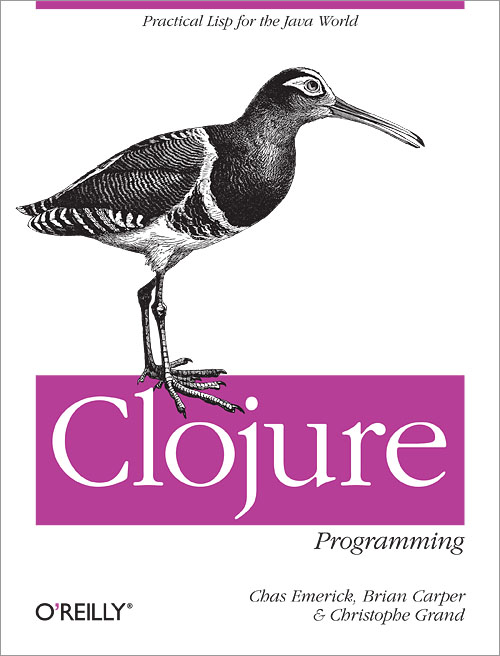
\includegraphics[height=4cm]{img/clj-prog}
      \end{block}
    \end{column}
    \begin{column}<3->{0.4\textwidth}
      \begin{block}{The Joy of Clojure}
        \centering
        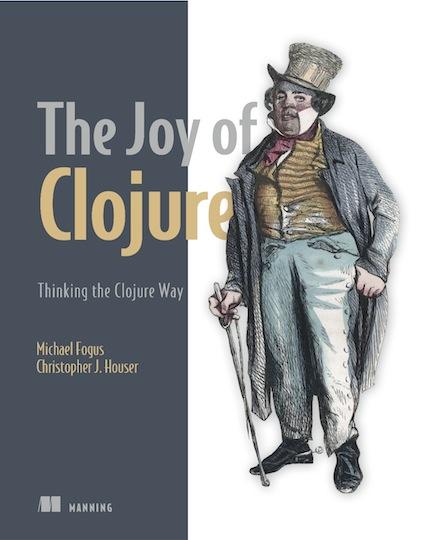
\includegraphics[height=4cm]{img/joy-of-clj}
      \end{block}
    \end{column}
  \end{columns}
\vspace{3mm}
\uncover<4->{Begge finnes på Amazon.}
\end{frame}

\subsection{HTML5 og Web}
\begin{frame}
  \frametitle{Webutvikling}

  Web er hipt og kult. Hvordan starter jeg med å lage en web-applikasjon i
  Clojure?

  \begin{itemize}
  \item<2-> 
\includegraphics[height=1cm]{img/noir} -
    \url{http://www.webnoir.org}
  \item<3-> 
\includegraphics[height=1cm]{img/korma} -
    \url{http://www.sqlkorma.com}
  \end{itemize}

  \vspace{3mm}
  \uncover<4->{Er lett å bruke for de med Python-bakgrunn.}
\end{frame}

\subsection{Miljø}
\begin{frame}
  \frametitle{Miljøet}
  Clojuremiljøet er veldig åpent og hyggelig

  \begin{itemize}
  \item<2-> IRC: {\tt \#clojure} på Freenode
  \item<3-> Epostlister: {\tt Clojure} og {\tt Clojure Dev} på Google Groups
  \item<4-> Biblioteker og rammeverk er det bare å bidra på
  \item<5-> Clojure Core - må sende inn Contributors Agreement. (Med andre ord
    litt tungvint)
  \end{itemize}
\end{frame}

\section{Avslutning}
\subsection{Spørsmål}
\begin{frame}
  \frametitle{Spørsmål}
  \begin{center}
    {\Huge Noen spørsmål?}
  \end{center}
\end{frame}

\subsection{Finish}
\begin{frame}
  \frametitle{Takk for meg}
  \begin{center}
    {\Huge Takk for oppmerksomheten!}
  \end{center}
\end{frame}

\end{document}
